% !TeX encoding = UTF-8
% !TeX spellcheck = en_US
% !TeX root = ../00_first_presentation.tex

%----------------------------------------------------------------
\begin{frame}{Frame 1}
\frametitle {Basic Navigation Tasks}
 
%\begin{columns} % contents are top vertically aligned
%\begin{column}{8cm} % each column can also be its own
\begin{block}{Scenario Environment}
\begin{itemize}
\item Walls, service areas, places, arena objects
\item Wall markers and floor markers
\item Obstacles
\end{itemize}
\end{block}  
 
%\end{column}
%\begin{column}{5cm} % alternative top-align that's better for graphics
	\centering
    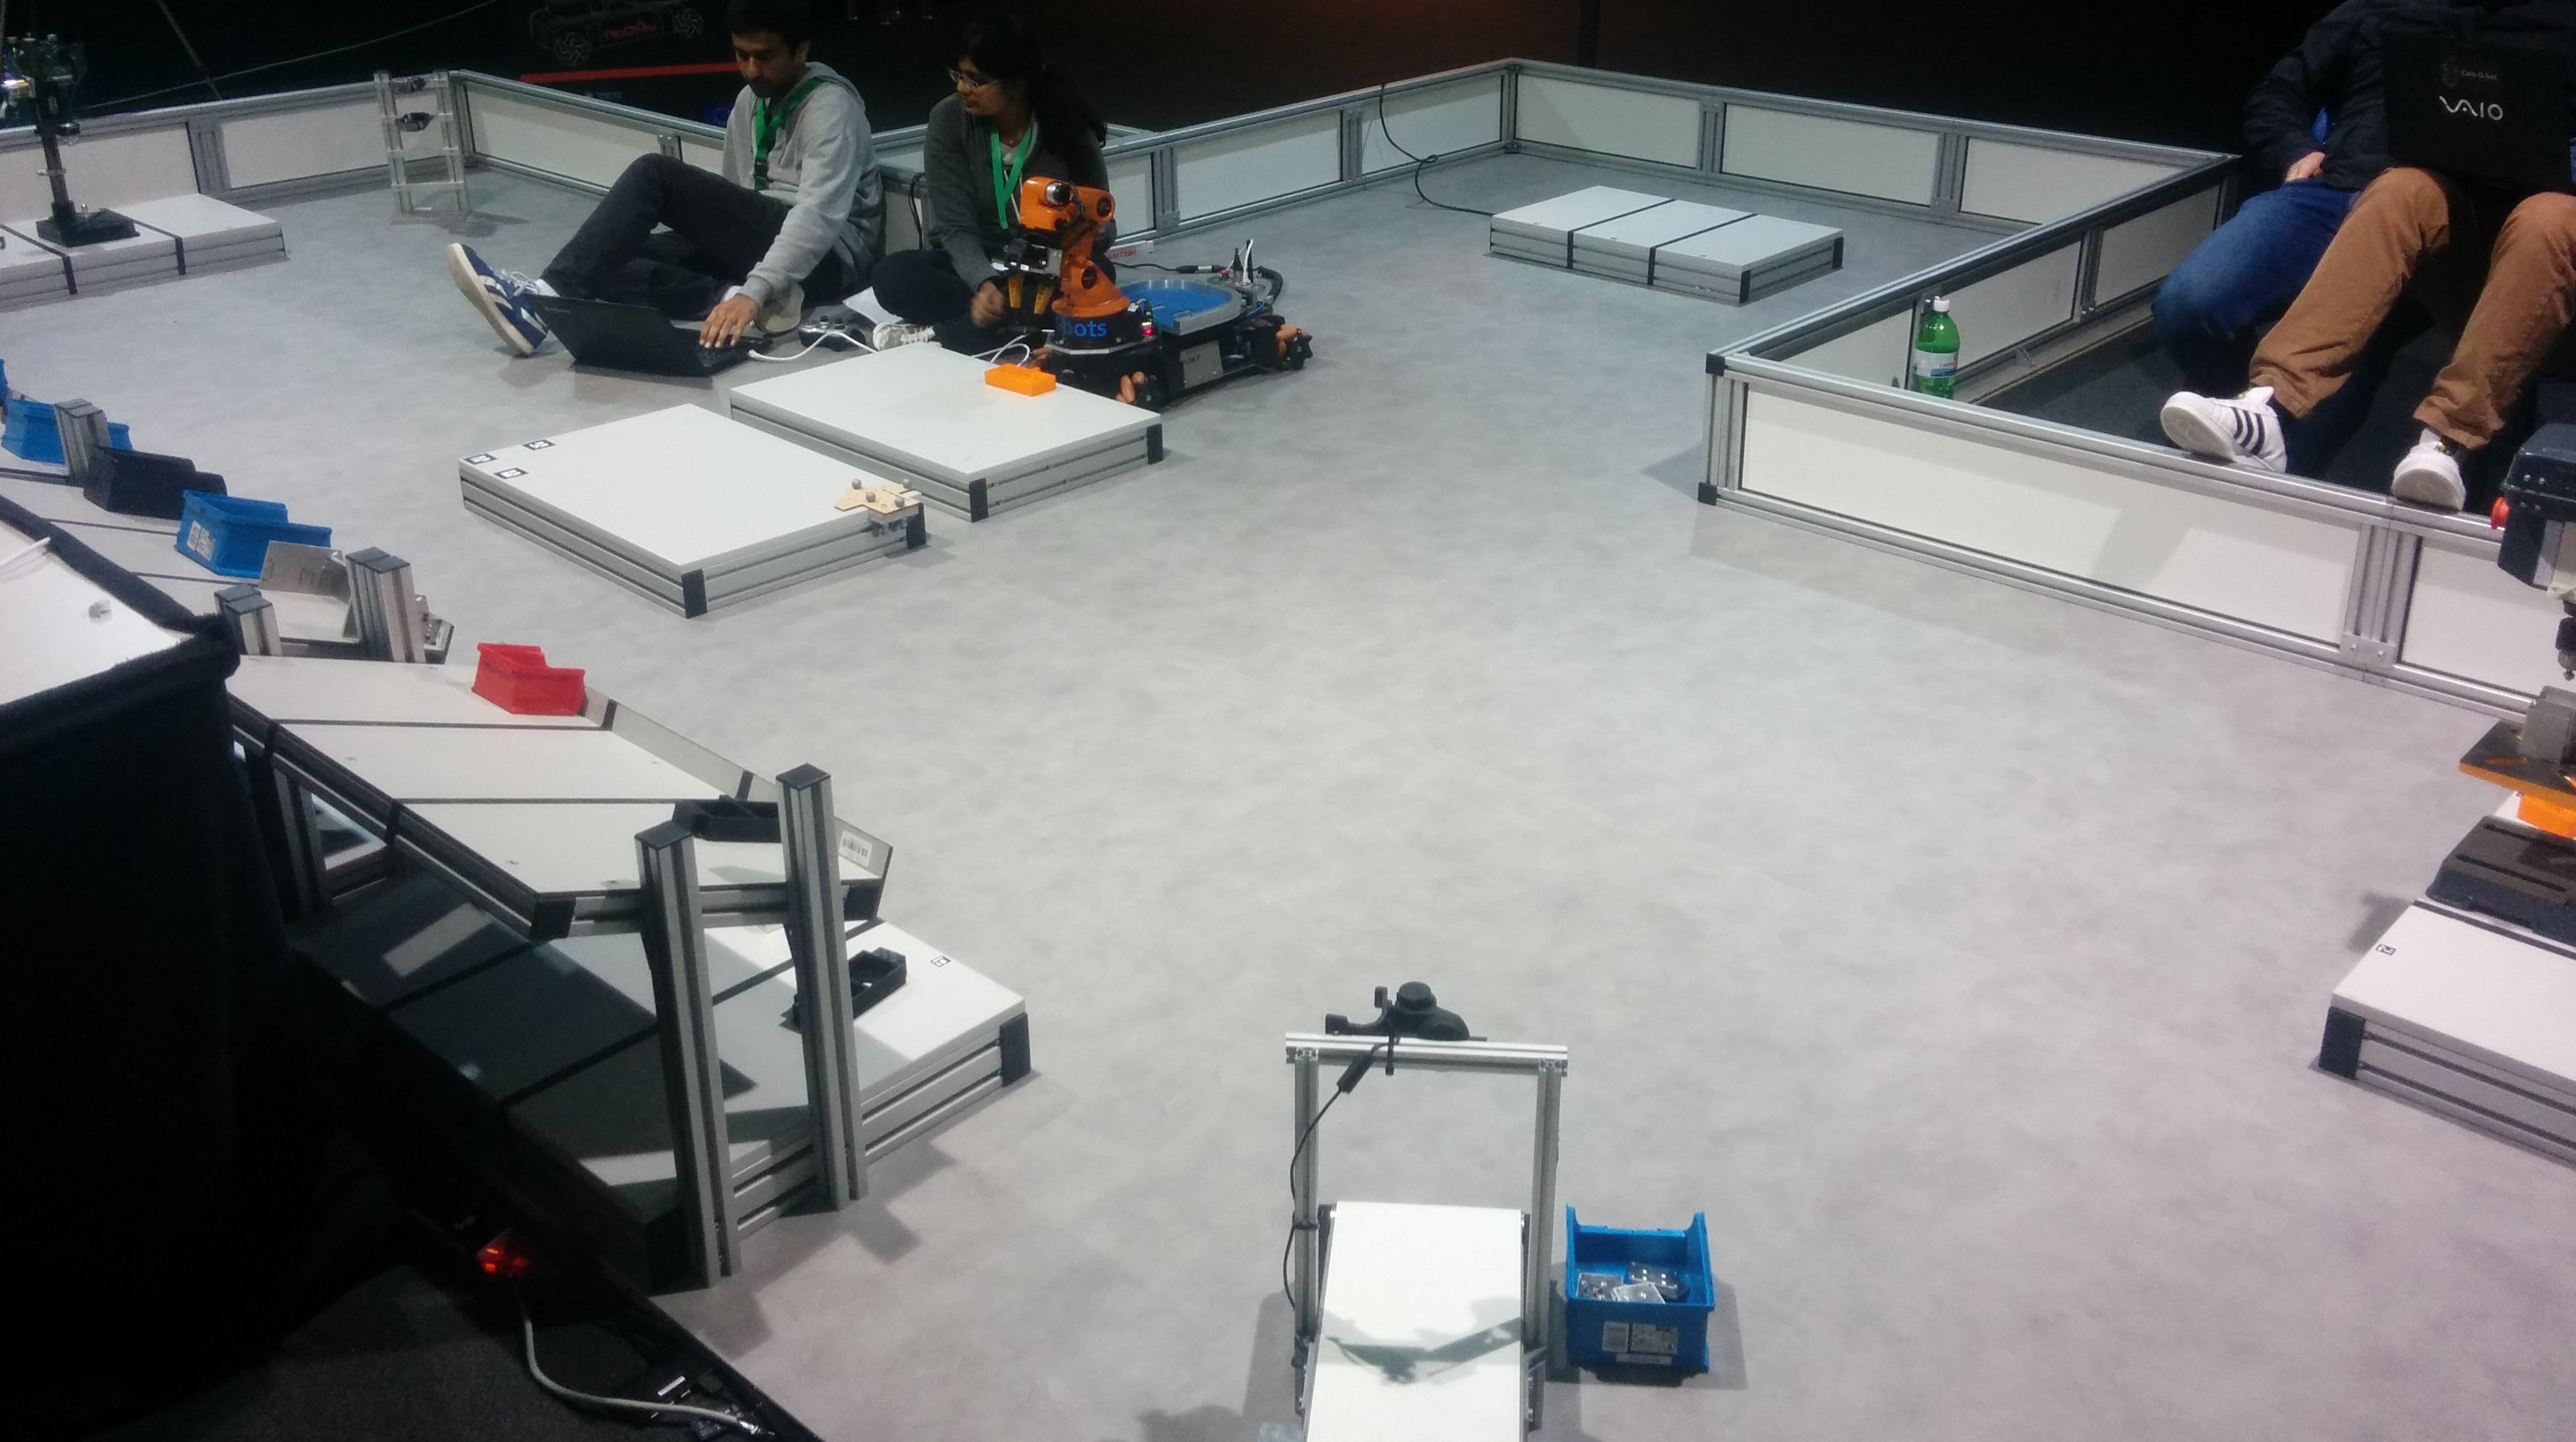
\includegraphics[height=40mm]{slides/gfx/arena.jpg}
%\end{column}
%\end{columns}
 
\end{frame}
%----------------------------------------------------------------
\begin{frame}{Frame 1}

\frametitle {Basic Navigation Tasks}
\begin{block}{Tasks}
	\begin{itemize}
		\item Task Specification
		\begin{itemize}
		\item Place
		\item Orientation
		\item Pause duration
\end{itemize}		   
		\item Purpose
		\begin{itemize}
		 \item Move to the places orderly 
		 \item Finally leave the arena through the gate
\end{itemize}		
		\item Requirement
		\begin{itemize}
		 \item Orient itself according to the orientation
		 \item Cover a place marker
		 \item Pause for the time in seconds
\end{itemize}		
	\end{itemize}
\end{block}    
 
\end{frame}
 %----------------------------------------------------------------
\begin{frame}{Navigation Subtasks and Challenges}

\begin{block}{Perception}
	\begin{itemize}
		\item Reading and processing sensor data
		\item \alert {Challenges}
		\begin{itemize}
		\item Sensor error
		\item Sensor calibration
		\item Sensor fusion 
		\item Interpreting markers
\end{itemize}		  
	\end{itemize}
\end{block}
\end{frame}
\begin{frame}{Navigation Subtasks and Challenges}

\begin{block}{Mapping}
	\begin{itemize}
		\item Building the map of environment
		\item \alert {Challenges}
		\begin{itemize}
		\item Measurement noise
		\item Dynamic environment 
		\item High dimension
		\item Barrier tape
\end{itemize}		
	\end{itemize}
\end{block}
 
\end{frame}
 %----------------------------------------------------------------
\begin{frame}{Navigation Subtasks and Challenges}

\begin{block}{Localization}
	\begin{itemize}
		\item Calculate current position in the map
		\item \alert{ Challenges}
		\begin{itemize}
		\item Dynamic environment
		\item Motion errors
		\item Similar surroundings 
\end{itemize}		  
	\end{itemize}
\end{block}
 
\end{frame}
%----------------------------------------------------------------
\begin{frame}{Navigation Subtasks and Challenges}

\begin{block}{Path planning}
    \begin{itemize}
    		\item Determine a sequence of actions from start to goal position.
    		\item Given: Map, start pose, goal pose, robot geometry
    		\item Map: representation, update
    		\item Types: Grid-based, Graph-based, Field-based
    		\item Search algorithms
    		\item \alert{Challenges: Accessibility problem, computational complexity, uncertainties, dynamic environment}
    \end{itemize}
\end{block}
\end{frame}
%----------------------------------------------------------------
\begin{frame}{Navigation Subtasks and Challenges}

\begin{block}{Motion control}
    \begin{itemize}
    		\item Subtasks: Path execution and acting
		\item Move robot from point to point or follows a trajectory
    		\item Input: Path commands, output: motor commands to wheels
    		\item Odometry feedback
    		\item Requirements: Kinematic model
    		\item Robot kinematics influences the maneuverability and controllability.
    		\item \alert{Challenges: System modeling complexity, system errors}
    \end{itemize}
\end{block}

\end{frame}